% based on scrbook
% finaler Ablauf: übersetzen, Tools -> Benutzer -> MakeNomenclature, übersetzen
\documentclass[
fontsize=12pt, %font size
paper=a4, %paper format
headsepline, %separating line for header
chapterprefix, % produce "Chapter ..."
numbers=noenddot, % no full-stop after last number
listof=totoc, %Entry in table of contents for list of figures/tables
index=totoc, %Entry in table of contents for index
bibliography=totoc, %Entry in table of contents for bibliography
%BCOR=5mm,%Binding correction, ensures sufficient space for binding
%todo change this to final to switch off for expamle the showlabels
%todo manually put 'disable' in front of usepackage{todonotes}
%final,%
]%
{scrbook}%

\KOMAoptions{twoside=false}




\usepackage{geometry}
\geometry{
a4paper,
total={150mm,205mm},
left=15mm,
right=50mm,
}

% 

% --------- Packages ----------
%\NeedsTeXFormat{LaTeX2e}
%\usepackage[dvips]{epsfig}
%\usepackage[latin1]{inputenc}
% TODO Argument "english" checken
\usepackage[english]{babel} 
%\usepackage[ngerman]{babel} 
\usepackage{a4wide}
%\usepackage{psfig}
\usepackage{fancyhdr}
\usepackage{latexsym}
\usepackage{enumerate}
\usepackage{paralist}
\usepackage{float}
\usepackage{verbatim}  % verbatiminput
\usepackage{caption}
\usepackage{floatflt}
\usepackage{afterpage}
\usepackage{graphicx}
\usepackage[space]{grffile}  % handles space in file name
\usepackage{moreverb}     
%\usepackage[]{mcode}
\usepackage{bbm}

% spacing of items: noitemsep 
\usepackage{enumitem}


% \usepackage{tabulary} % to set dith to side width and use left/right alignment
%\usepackage{showframe} % show margin of page


\usepackage[intoc]{nomencl}
\makenomenclature

% math
\usepackage{mathtools} % successor of \usepackage{amsmath}
\usepackage{amssymb,amsfonts}
\setcounter{MaxMatrixCols}{10} % leftover from Marcos
\usepackage{cases}

% Pseudo Code
\usepackage{algorithm}
\usepackage[noend]{algpseudocode}

%% bibliography
%%\usepackage[style=authoryear, backend=biber]{biblatex}
%%%\usepackage{biblatex}
%%\bibliography{bib}
%\usepackage[round, sort, comma]{natbib}
%\bibliographystyle{apalike}


% fraction for floats
\renewcommand{\floatpagefraction}{0.8}
%\renewcommand{\textfraction}{0.15}


% prevent floats from floating too much around (stay in one section)
%\usepackage[section]{placeins}

% adjust font of abbreviations
\usepackage{helvet}
\renewcommand{\nomlabel}[1]{{\fontfamily{phv}\selectfont \textbf{#1}}} %bold Helvetica



% ---------------------------------------------------------------------------------------------
% OWN PACKAGES 
% ---------------------------------------------------------------------------------------------

% tables
\usepackage{booktabs}
\usepackage{longtable}
\usepackage{tabularx} % especially for the title page
\newcolumntype{L}{>{\raggedright\arraybackslash}X}
\newcolumntype{Y}{>{\centering\arraybackslash}X}
\newcolumntype{R}{>{\raggedleft\arraybackslash}X}
\newcolumntype{x}{>{$}l<{$}} % math-mode version of "l" column type
\newcolumntype{y}{>{$}c<{$}} % math-mode version of "c" column type
\newcolumntype{z}{>{$}r<{$}} % math-mode version of "r" column type

\usepackage{multicol}



% language
\usepackage[utf8]{inputenc} % to type ä,ö,ü,...


% fast text
\usepackage{lipsum}

% bibliography
\usepackage[round, sort, comma]{natbib}
\bibliographystyle{apalike}

\usepackage{color}
\usepackage[dvipsnames]{xcolor}


% quotes
\usepackage{csquotes}
\usepackage[%
%	allbordercolors=black,
urlcolor=blue,
linkcolor=blue,
citecolor=.
]{hyperref}
\usepackage{cleveref}


% to show the assigned labels
% has to be included after the packages amsmath and hyperref
\usepackage{showlabels}

% todo
\usepackage%
[textwidth=40mm,
draft,%
%disable%
]%
{todonotes}


\usepackage{float}

%bold math symbols
\usepackage{bm}

% multiple figures
\usepackage{subcaption}


\usepackage[onehalfspacing]{setspace}

\usepackage{pdfpages}
% switched to .tex as then commands are directly included in AutoFill

% own package
% https://www.sharelatex.com/learn/Writing_your_own_package#Options

\NeedsTeXFormat{LaTeX2e}
\ProvidesPackage{z-style}


% colours
\RequirePackage[dvipsnames]{xcolor}
\definecolor{colStefan}{HTML}{e68a00}
\definecolor{colIdea}{HTML}{00cc00}

\RequirePackage{xstring} % for if statements


%todoNotes
\newcommand{\todoBib}[1]{\todo[color=green!40]{#1}}
%\newcommand{\todoRed}[2][noinline]{\todo[color=red!40, #1]{#2}}
\newcommand{\todoRed}[1]{\todo[inline, color=red!40]{#1}}
\newcommand{\todoMinor}[1]{\todo[inline, color=orange!20]{#1}}
\newcommand{\todoCurrentWork}[1]{\todo[inline, color=red!60]{CURRENTLY WORKING HERE: #1}\vspace*{5cm}}
\newcommand{\todoRequirememnt}[1]{\todo[color=cyan!10]{#1}}

% nice graphic for network example
\usetikzlibrary{arrows.meta,positioning}



% nicer coloured box
% https://tex.stackexchange.com/questions/66154/how-to-construct-a-coloured-box-with-rounded-corners
\usepackage[most]{tcolorbox}
\RequirePackage{tcolorbox}
\newtcolorbox{boxStefan}{colback=colStefan!5!white,colframe=colStefan!90}
\newtcolorbox{boxIdea}{colback=colIdea!5!white,colframe=colIdea!90}


% some often used typography
\newcommand{\eg}{\mbox{e.\,g.}\xspace}
\newcommand{\ie}{\mbox{i.\,e.}\xspace}
\newcommand{\wlogMath}{\mbox{w.\,l.\,o.\,g.}\xspace}

% ------------------------------------------------------------------------------
% Theorem-Umgebungen
\theoremnumbering{arabic}%

% first block

\theoremheaderfont{\bfseries}%
%\theorembodyfont{\upshape}%
%\theoremseparator{}%
\theorembodyfont{\normalfont}%
\theoremseparator{.}

\newtheorem{theorem}{Theorem}%
\crefname{theorem}{Theorem}{Theorems}
\Crefname{theorem}{Theorem}{Theorems}
\newtheorem{lemma}[theorem]{Lemma}%
\crefname{lemma}{Lemma}{Lemmas}
\Crefname{lemma}{Lemma}{Lemmas}
\newtheorem{definition}[theorem]{Definition}%
\crefname{definition}{Definition}{Definitions}
\Crefname{definition}{Definition}{Definitions}
\newtheorem{remark}[theorem]{Remark}%
\crefname{remark}{Remark}{Remarks}
\Crefname{remark}{Remark}{Remarks}

% second block

\theoremstyle{nonumberplain}%
\theoremheaderfont{\bfseries}%
\theorembodyfont{\normalfont}%
\theoremseparator{.}
\theoremsymbol{\ensuremath{\Box}}% ensuremath -> sowohl im Text- als auch im Mathemodus wird das gewünschte Zeichen gesetzt

\newtheorem{proof}{Proof}%
\crefname{proof}{Proof}{Proofs}
\Crefname{proof}{Proof}{Proofs}
% ------------------------------------------------------------------------------
%\newenvironment{proof}[1][Proof]{\noindent\textbf{#1.} }{\ \rule{0.5em}{0.5em}}
%\textwidth =170mm
%\textheight=205mm
%\oddsidemargin=-8mm
%\evensidemargin=-8mm
\DeclareMathOperator*{\argmax}{arg\,max}
\DeclareMathOperator*{\argmin}{arg\,min}

\title{Reinforcement Learning and Artificial Intelligence\\
	in the context of revenue management}

% ------------------------------------------------------------------------------
% PDF-Metadaten
\hypersetup{
	pdfauthor={Stefan Glogger},
	pdftitle={\Title},
	pdfsubject={},
	pdfkeywords={Master's Thesis, Revenue Management, Approximate Dynamic Programming, Neural Networks, Machine Learning},
	%todo adopt this for print version
	colorlinks=true, %coloured links (for the PDF version)
	% colorlinks=false, % no coloured links (for the print version)
}
% ------------------------------------------------------------------------------

\usepackage{adjustbox}

\begin{document}

\listoffigures
\listoftables

%\chapter{Introduction}

\begin{enumerate}[noitemsep]
	\item Entstehung Revenue Management
	\item klassische Annahme des independent demand greift zu kurz
	\item stattdessen Modellierung von Customer Behaviour
	\item Problem des Customer Control Based Revenue Managements
	\item Relevanz von Revenue Management
	\item Weitere Fragen, mit denen sich RM beschäftigt
	\item Ziel der Arbeit
	\item Kurzüberblick der Kapitel
\end{enumerate}

The concept of revenue management originated as a result of the U.S. Airline Deregulation Act of 1978 \cite{Talluri.2005}. Prior to this, prices had been strictly controlled and standardized by the U.S. Civil Aviation Board (CAB\nomenclature{CAB}{U.S. Civil Aviation Board}). Afterwards, airlines were free to choose prices, change schedules and alter offered services at their will, without CAB approval. This deregulation resulted in the immediate appearance of low-cost/no-frill airlines. By operating on lower labour costs and less service on board, profitable fares up to $70 \%$ lower than the ones of major carriers could be offered and an market pressure on classical large airlines increased. They now faced the problem of which price to offer at any given circumstances. 

The traditional, rather simple assumption of independent demand didn't work. It expects demand to be independent of the current market conditions such as prices offered by competitors, (day-)time of departure, frequency of departures or brand image \cite{Talluri.2005}. Furthermore, low fare demand is generally expected to come before high fare demand (as business travellers prefer the flexibility to possibly change their schedule). The problem reduced to: How much capacity should be reserved for the high fare demand, that appears later? But as the purchase of a ticket clearly depends on the market situation (e.g. an exceptional Formula 1 race at one specific weekend) or the continuing expansion of low-cost airlines offering undifferentiated fare structures, this simple assumption of independent falls short in practice \cite{Bront.2009}.

As a result, academia shifted its focus to more sophisticated models building on customer choice behaviour. Demand is assumed to depend on the currently offered products, which might change depending on the circumstances. This assumption now allows to also account for buy-up (buying a higher fare when lower fares are closed) and buy-down (switching to a lower fare when discounts are available). The assumption of customer choice is then incorporated in dynamic pricing models, as e.g. studied by \cite{Gallego.1997}, \cite{Bitran.1998} or \cite{Feng.2000}.

The underlying problem is referred to as capacity control under customer choice behaviour and can be summarized as: Which products should be offered at any given circumstance, whereby circumstance is determined mainly by time to departure and remaining capacity. As many airlines operate so called hub-and-spoke networks, allowing them to offer service in many more markets than with point-to point connection, the problem becomes more challenging \cite{Talluri.2005}. This is incorporated by modelling each point-to-point connection (single leg) by one separate resource and each seat as one unit of capacity. Furthermore, different customers (e.g. business vs. leisure traveller) can be distinguished by modelling them as different customer segments. Thus, the central problem in capacity control can be stated as:

\begin{center}
	\emph{Given a network consisting of several flights (edges) connecting certain cities (vertices) with varying seat capacity (weight of edge) and given a certain time to departure, which combination of products shall be offered to the customers?}
\end{center} 

Note that revenue management is relevant in many fields, even though we introduced the problems purely in the airline setting. The introduction was done intentionally like this as revenue management is closely connected to the airline industry and it increases total profitability by $4$ to $5 \%$ of revenues \cite{Talluri.2005}\footnote{We want to point out that Soutwest Airlines is often mentioned as a counterexample. But even though its pricing structure is very simple, revenue management systems are still used \cite{Talluri.2005}.}. However, revenue management appears in any decision related to demand management. and \cite{Talluri.2005} structured those decisions in three basic categories:

\begin{itemize}
	\item Structural decisions: How the selling process is organized (e.g. negotiations among individuals, auctions with restricted access, publicly posted prices) or how additional terms are structured (e.g. volume discounts or refund options).
	\item Price decisions: How to set individual offer prices, reserve prices (in auctions) and posted prices or how to price over time.
	\item Quantity decisions: Whether an offer to buy should be accepted or rejected or when to withhold a product from the market in order to sell it at a later point in time.
\end{itemize}

With this general framework and the relevance of revenue management in mind, we can formulate the goal of this thesis. We want to explore different methods of \enquote{solving} the capacity control problem under choice behaviour in the single-leg and multi-leg setting by implementing the algorithms in Python, let them cope with exemplary test scenarios and compare their performance. Furthermore, new methods such as the usage of Neural Networks shall be discussed and evaluated. 

The remaining of the thesis is structured as follows. 
\Cref{ch:Literature} gives an overview of existing literature.
\Cref{ch:ProblemsMethods} describes the problem formally and introduces various solution methods.
\Cref{ch:ComparisonTheory} presents theory on how to compare different methods based on statistics.
\Cref{ch:Examples} evaluates the different methods in one single-leg and one multi-leg scenario.
Finally, \Cref{ch:conclusion} summarizes the thesis and presents an outlook for future research. The code of the implementation is given in \Cref{ch:code} but can also be found on \todo{LM: Referenz zum Code überprüfen}\todo{GitHub repository für Abgabe der Masterarbeit}.


%% !TeX root = ADP-SG.tex

\chapter{Problem and Approaches to Solution}\label{ch:ProblemsMethods}

This chapter introduces the classical revenue management problem of capacity control problem under customer choice behaviour as can be found e.g. in \cite{Koch.2017} or in \cite{Strauss.2018}. It consists of deciding which products to offer at a given point in time and \Cref{s:Prob} gives a general description of the problem as well as a formulation as a dynamic program. Various methods of solving the problem are laid out in \Cref{s:Metho}.

\section{The problem}\label{s:Prob}

In this section, we describe the capacity control in general in \Cref{ss:Prob:GenDesc}, present a concrete example in the airline setting in \Cref{ss:Prob:AirDesc} and introduce the formulation of the resulting choice based capacity control model as a dynamic program in \Cref{ss:Prob:FormDynProg}. \todo{Subsection zu Problemen in der Lösung einfügen, die überleitet zu den verschiedenen Lösungsmethoden}

\subsection{General description}\label{ss:Prob:GenDesc}

A company offers a bundle of products to heterogeneous customers arriving over time. Products often correspond to services that have to be delivered at a given point in time. The period of time from now until delivery is referred to as selling horizon (or booking horizon), is considered finite and is split into a finite set of consecutive time points. The set of available products is also assumed to be finite and without loss of generality (w.l.o.g.\nomenclature{w.l.o.g.}{without loss of generality}) constant over time\footnote{If the set of available products change over time, let $S_t$ denote the set of available products at time $t$ and let $\mathcal{T}$ represent the finite set of time points. Then, $S \coloneq \cup_{t \in \mathcal{T}}S_t$ is again finite (finite union of finite sets) and can be taken as the constant set of available products at each time point.}. Each individual product is characterized by a given price and usage of a certain, finite, set of resources. These resources might be shared among different products. 

The goal of companies operating in the capitalistic society is to increase profits, which is equivalent to maximizing revenue in a specific setting. As stated, the price of individual products (leading to revenue) is assumed to be fixed, which is a realistic assumption for short terms considering potentially large costs coming with a change of price (e.g. selling products via catalogue). Furthermore, capacities are fixed in the short term (costly to increase production as e.g. more employees have to be hired) and are considered perishable. Often, capacity comes with high fixed costs and low marginal costs resulting from selling an additional product at any price (e.g. costs for operating one flight with 97 customers are mostly the same as for operating the same flight with 98 customers). Such a profit and cost structure justify the usage of revenue as a proxy for profit \cite{Strauss.2018}.

Switching to the customer side, the consideration of a heterogeneous customer group allows for modelling most real world scenarios. Not every customer is the same, but it is certainly reasonable to combine individuals to groups sharing similar characteristics. Some characteristics will be more prevalent in the overall population (more precise, the population that represents all persons interested in the companies' products).  Different customers have varying needs, thus different preferences and different willingness-to-pay leading ultimately to different purchases depending on the currently offered set of products. Thus, the company can influence the sales process by altering the offered set of products over the booking horizon, which is exactly the task of capacity control under customer choice behaviour.

\subsection{Description in airline setting}\label{ss:Prob:AirDesc}

An airline company operates a flight network connecting cities A, B and C as depicted in \Cref{fig:AirDesc}. The booking horizon consists of 20 time steps (e.g. today is Monday, booking is possible four times every day until and including Friday and flights depart on Saturday). The products to be offered are summarized in \Cref{tb:AirDesc:Prod}. Note that two products are available on Leg 1, i.e. the expensive product 1 and the less expensive product 2 (e.g. due to separate business and economy classes). A sell of either product 1 or product 2 will result in the reduction of available capacity on Leg 1 by one unit. Furthermore, product 6 presents an option to get from city A to city C (via city B) and thus a sell of product 6 results in a reduction of both Leg 1 and Leg 2 by one unit. Also product 4 is connecting city A and city C (on the direct flight) but is more expensive then product 6 (e.g. the company assumes the shorter travel time is of value to some travellers). 

Furthermore, capacities are presented in \Cref{tb:AirDesc:Res}, so there are eight available seats on Leg 1, but just four seats are available on Leg 2. Customers are characterized as stated in \Cref{tb:AirDesc:Cust}, so most customers belong to segment 1 (higher value of $\lambda_l$ representing larger size of customer segment $l$) and want to travel from city A to city B and prefer the budget option (as the value of preference for the latter product is much higher and a higher value corresponds to a higher preference). Customers belonging to segment 2 also want to travel from A to B, but are price insensitive, as they value the higher comfort of the more expensive product 1 just little higher as the cheaper product 2. Business customers that need to travel from A to C are represented by customer segment 3 as can be seen by the low preference for no purchase. 

\todo{Layout: bring the figure and all tables into one floating element, or one figure stating the whole example (including time maybe in caption)}
\begin{figure}
	\caption{Airline network for description of capacity control problem. \label{fig:AirDesc}}
	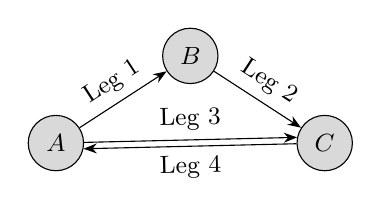
\begin{tikzpicture}[
	mycircle/.style={
		circle,
		draw=black,
		fill=gray,
		fill opacity = 0.3,
		text opacity=1,
		inner sep=0pt,
		minimum size=20pt,
		font=\small},
	myarrow/.style={-Stealth},
	node distance=0.6cm and 1.2cm
	]
	\node[mycircle] (cB) {$B$};
	\node[mycircle,below left=of cB] (cA) {$A$};
	\node[mycircle,below right=of cB] (cC) {$C$};
	
	\foreach \i/\j/\txt/\p in {% start node/end node/text/position
		cA/cB/Leg 1/above,
		cB/cC/Leg 2/above}
	\draw [myarrow] (\i) -- node[sloped,font=\small,\p] {\txt} (\j);
	\draw[myarrow]([yshift= 20pt] cA) -- node[sloped,font=\small,above] {Leg 3} ([yshift= 20pt] cC);
	\draw[myarrow]([yshift= -20pt] cC) -- node[sloped,font=\small,below] {Leg 4} ([yshift= -20pt] cA);
	\end{tikzpicture}
\end{figure}

\begin{table}
	\caption{Airline network for description of capacity control problem (products). \label{tb:AirDesc:Prod}}
	\begin{tabular}{yxz}
		\toprule
		\text{Product} & \text{Origin-destination} & \text{Fare}\\
		\midrule
		1 & A \rightarrow B & 5\\
		2 & A \rightarrow B & 3\\
		3 & B \rightarrow C & 5\\
		4 & A \rightarrow C & 12\\
		5 & C \rightarrow A & 10\\
		6 & A \rightarrow B \rightarrow C & 8\\
		\bottomrule
	\end{tabular}
\end{table}

\begin{table}
	\caption{Airline network for description of capacity control problem (resources). \label{tb:AirDesc:Res}}
	\begin{tabular}{yy}
		\toprule
		\text{Leg} & \text{Capacity}\\
		\midrule
		1 & 8\\
		2 & 4\\
		3 & 4\\
		4 & 8\\
		\bottomrule
	\end{tabular}
\end{table}

\todo{Idee: Beschreibung der Customer Segmente könnte man zu \enquote{Persona} ausweiten}
\begin{table}
	\caption{Airline network for description of capacity control problem (customers).\label{tb:AirDesc:Cust}}
	\begin{tabular}{lccccc}
		\toprule
		Segment & $\lambda_l$ & Consideration tuple\footnote{Note that in contrast to \cite{Bront.2009}, we use the mathematically correct terminology as \emph{tuple} does have an inherent order, while \emph{set} does not (and thus makes no mathematical sense to be combined with a preference vector referring to the order of products in the set).} & Preference vector & No purchase preference & Description\\
		\midrule
		1 & $0.3$ & $(1, 2)$ & $(4, 8)$ & $2$ & Price sensitive, (A$\rightarrow$B)\\
		2 & $0.2$ & $(1, 2)$ & $(6, 5)$ & $2$ & Price insensitive, (A$\rightarrow$B)\\
		3 & $0.2$ & $(4, 6)$ & $(8, 4)$ & $1$ & Price sensitive, fast (A$\rightarrow$C)\\
		4 & $0.1$ & $(5)$ & $(2)$ & $2$ & Opportunity traveller, (C$\rightarrow$A)\\
		\bottomrule
	\end{tabular}
\end{table}

\subsection{Formulation as dynamic program}\label{ss:Prob:FormDynProg}

\subsubsection{Firm's perspective}

\begin{boxStefan}
	\begin{enumerate}
		\item time index always at the top
		\item index for products always at bottom
	\end{enumerate}

	Anständiges Symbolverzeichnis, z.B. mit glossaries \url{https://ctan.org/pkg/glossaries}
	
	Wertebereich der Variablen
\end{boxStefan}

\todo{Übersichtsliteratur \cite{Phillips.2011} anschauen (nur an Uni Augsburg, nicht an TUM)}

Extensive literature deals with revenue management and came up with formal notation suitable for the analysis of capacity control models. Good overviews can be found in \cite{Klein.2008} or in \cite{Phillips.2011}. In this thesis, we introduce notation for a capacity control model first under a general discrete choice model of demand and then directly using a multinomial logit model of demand. Notation is closely linked to \cite{Koch.2017} and the standard representation is used for a better orientation with the main ideas outlined in \Cref{tb:Prob:Notation}

\todo{Idee: Notation vereinheitlichen, stets ähnlich zu $t=1, \dots, T$. Also z.B. statt $j=1,\dots,n$ für Produkte auch $j=1,\dots,J$}
\todo{Notation: Change transpose to $\backslash$ text\{T\}}
\begin{table}
	\caption{Idea of notation}\label{tb:Prob:Notation}
	\begin{tabular}{cll}
		\toprule
		Symbol & Characteristic & Meaning\\
		\midrule
		$i, j, h, t, l, p$ & general small letter & index\\
		$n, m$ & specific small letters & maximum index\\
		$T, L$ & general capital letter & maximum index\\
		$S$ & {\color{red}specific capital letter} & tuple of elements\\
		$x_1$ & small with index & single number\\
		$\boldsymbol{x}$ & small and bold & vector\\
		$(x_1, \dots, x_n)$ & parenthesis around single numbers & row vector\\
		$(\dots)^T$ & $T$ on upper side & transpose\\
		
	\end{tabular}
\end{table}

First, we present the situation with its inflexible components. Consider a firm that produces $n$ distinguishable products indexed by $j = 1, \dots, n$. We already introduce the notation $[n] \coloneqq \{1, \dots, n\}$. Product $j$ comes with a certain price leading to a revenue of $r_j$ when the product is sold. The revenues are bundled by the vector $\boldsymbol{r} = (r_1, \dots, r_n)^T$. A total of $m$ different resources are used for production, which are indexed by  $h \in [m]$. In order to produce one unit of product $j$, certain resources are needed and the consumption of resources is captured by the vector $\boldsymbol{a}_j = (a_{1j}, \dots, a_{mj})^T$ are necessary, with $a_{hj}=1$ if resource $h$ is needed for production of product $j$ and $a_{hj} = 0$ otherwise. The resource consumption can be aggregated in the incidence matrix $A = (a_{hj})_{h\in [m], j \in [n]}\in {0, 1}^{m \times n}$. Additionally, the firm already identified the group of potential customers and segmented this group into a total of $L$ customer segments, which are indexed by $l \in [L]$. A customer of segment $l$ arrives with probability $\lambda_l$ and this parameter can be adjusted such that it matches the reality (e.g. there are two times as many customers belonging to segment $a$ then there are of segment $b$, so we choose $\lambda_a = 2\lambda_b$ ) and the model assumptions (only one customer arrives during each period).
\todo{Skalierung und Einflüsse auf Ankunftsraten in Fußnote oder Appendix}
\todo{Ergänzung: Beweis zu arrival probabilities können aufsummiert als kleiner gleich 1 angenommen werden, da der Parameter eines Poisson Prozesses dessen erwartete Ankunftszeit (? eig höher => mehr Leute kommen) beschreibt und damit mit der Feinheit der Zeitschritte angepasst werden kann. Poisson Prozess in \cite{Bront.2009} 3. Model }. 

The finite time period from when booking is possible for the first time to when it is possible for the last time is discretized into a total of $T$ sufficiently small time periods, such that in each individual time period at most one customer arrives. Time periods are indexed by $t \in [T]$. To be very precise (particularly relevant for correct implementation), booking itself is just possible at beginning of each time period, i.e. for time period $t$, booking is possible at time point $t-1$. Furthermore, one customer purchases at most one product. 

Second, we look at the flexible components of the model, i.e. those components that might change over time. Initially, i.e. at the start of the first time period (time point 0), the available capacity of resource $h$ is given by $c_h^0$ and thus all available capacities are described by the vector $\boldsymbol{c}^0 = (c_1^0, \dots, c_m^0)^T$. 

Let us now explore what happens if product $j$ is purchased during time period $t$, i.e. at time point $t-1$. The old capacity vector is given by $\boldsymbol{c}^{t-1}$. As product $j$ claims capacities according to $\boldsymbol{a}_j$,  the capacity vector reduces accordingly to $\boldsymbol{c}^{t} = \boldsymbol{c}^{t-1} - \boldsymbol{a}_j$. Time moves forward, such that the last selling might occur at time period $T$, i.e. at time point $T-1$.

\todo{Grafik in tikz erstellen mit Übersicht zu wie läuft ein exemplarischer Verkaufsprozess ab}
\begin{figure}
	\centering
	\caption{Visualization of the booking horizon with its time periods.\label{fig:Prob:Horizon}}
	\includegraphics[width=0.7\linewidth]{NotizLoeschenBookingHorizon}
	\caption{}
	\label{fig:notizloeschenbookinghorizon}
\end{figure}


\clearpage
\setcounter{page}{1}
\noindent\fbox{\parbox{\textwidth}{\centering 26.8.}}

To sum it up, the firm aims at increasing the value of the products sold and has flexibility in the sets offered. Thus, the decision variables for each time period $t \in [T]$ are given by $\boldsymbol{x}^t = (x^t_1, \dots, x^t_n)^T$ with $x^t_j = 1$ if product $j$ is offered during time period $t$ (i.e. chosen at time point $t-1$) and $x^t_j = 0$ otherwise. Thus, for each time period $t$ and the prevalent capacity $\boldsymbol{c}$, the offer set $\boldsymbol{x}$ has to be determined. Note that in machine learning terms, this mapping is defined as a policy $\boldsymbol{\psi} = (\psi^1, \dots, \psi^T)^T$.\todo{ML-Notation hier anfügen oder wo?}

We can put the above in formulas after introducing the random variable $X^t$ as the product which is purchased at time point $t$, with the notation $X^t=\{0\}$ if no purchase is made at time point $t$. 
So we use $\Omega \coloneqq {0, 1, \dots n}$ as the underlying set (no purchase plus purchasable products) and can use $\sigma(\Omega)$ as underlying sigma algebra (note that $\Omega$ is finite by assumption). 
Furthermore, we introduce a probability measure $p_{\boldsymbol{x}^t}(\cdot)$ 
and use the shorthand $p_{\boldsymbol{x}^t}(j) = p_{\boldsymbol{x}^t}(\{j\}) = p_{\boldsymbol{x}^t}(X^t = \{j\})$ as the probability of product $j$ being purchased at time point $t$ when tuple $\boldsymbol{x}^t$ is offered. Note that, $p$ being a probability measure, it has to satisfy the corresponding Kolmogorov axioms 
\todo{Zitation einfügen}
\begin{alignat}{2}
p_{\boldsymbol{x}^t}(j) &\geq 0 \quad \forall j \in \{1, \dots n\} \quad &&\text{(non-negativity)}\\
p_{\boldsymbol{x}^t}(X^t \in \Omega) &= 1 &&\text{(unitarity)}\\
p_{\boldsymbol{x}^t}(\cup_{j \in J}\{j\}) &= \sum_{j \in J}p_{\boldsymbol{x}^t}(j) \quad \forall J \subset \Omega \quad &&\text{(additivity in discrete setting)}
\end{alignat}

How to arrive at those probabilities is discussed in \Cref{sss:DCM}. Now, we formalize the aim of the firm and bridge the connection to expectation theory. The expected revenue-to-go starting with time period $t$ and capacity $\boldsymbol{c}$ is given by the value function, which maximizes the expected revenue and is mostly formulated recursively because of complicated evolutions due to capacities changing over time.

%todo Verbindung zu Erwartungswert herstellen
%&= \max_{x^t \in \{0,1\}^n}\left\{ \mathbb{E}_{\boldsymbol{x}^t}(r_{X^t})\right\}\\

\begin{align}
V(t, \boldsymbol{c}) &= \max_{x^t \in \{0,1\}^n}\left\{ \sum_{j \in [n]} p_{\boldsymbol{x}^t}(j) \left( r_j + V(t+1, \boldsymbol{c} - \boldsymbol{a}_j) \right) + p_{\boldsymbol{x}^t}(0) V(t+1, \boldsymbol{c}) \right\} \label{eq:Bellman}\\
&= \max_{x^t \in \{0,1\}^n}\left\{ \sum_{j \in [n]} p_{\boldsymbol{x}^t}(j) \left( r_j - \Delta_j V(t+1, \boldsymbol{c}) \right) \right\} + V(t+1, \boldsymbol{c})\quad \forall t \in [T], \boldsymbol{c} \geq 0
\end{align}

with $\Delta_j V(t+1, \boldsymbol{c}) \coloneqq V(t+1, \boldsymbol{c}) - V(t+1, \boldsymbol{c} - \boldsymbol{a}_j)$ and boundary conditions $V(T+1, \boldsymbol{c}) = 0$ if $\boldsymbol{c} \geq \boldsymbol{0}$ and $V(t, \boldsymbol{c}) = - \infty \quad \forall t \in [T+1]$ if $\boldsymbol{c} \ngeq \boldsymbol{0}$, i.e. $\exists h \in [m]: c_h < 0$.

The optimal offerset $\hat{\boldsymbol{x}}^t$ is then given by

\begin{align}
\hat{\boldsymbol{x}}^t = \argmax_{x^t \in \{0,1\}^n}\left\{ \sum_{j \in [n]} p_{\boldsymbol{x}^t}(j) \left( r_j - \Delta_j V(t+1, \boldsymbol{c}) \right) \right\} + V(t+1, \boldsymbol{c})\quad \forall t \in [T], \boldsymbol{c} \geq 0\label{eq:DP-optOffer}
\end{align}


\subsubsection{Discrete Choice Model for Customer Behaviour}\label{sss:DCM}

\todo{formaler einführen mit \cite{Train.2009} und \cite{Talluri.2004}}

We already discussed that at each time period at most one customer arrives (out of $L$ customer segments), who can purchase at most one product. The only remaining question is which product is being purchased in a particular time period. There exist multiple models to describe purchase probabilities, but many of them are based on preferences in accordance with utility. We first introduce the utility concept in general and then introduce the multinomial logit model (MNL\nomenclature{MNL}{multinomial logit model}).

Consider customer segment $l$. Let $u_{lj} \in \mathbb{R}^+_0 \quad \forall j \in [n]$, resp. $u_{l0} \in \mathbb{R}^+$ denote the utility that a customer of segment $l$ assigns to product $j$, resp. to the no-purchase alternative. Then, the purchase probability of product $j$ given offer tuple $\boldsymbol{x}^t$ is given by $p_{l\boldsymbol{x}^t}(j)$, where again $p_{l\boldsymbol{x}^t}(0)$ denotes the probability of no purchase. In the MNL, the probabilities are derived by the following formulas

\begin{alignat}{2}
	p_{l\boldsymbol{x}^t}(j) &= \frac{u_{lj}x_j}{u_{l0} + \sum_{p\in[n]} u_{lp}x_p} \quad \forall j \in [n]\quad  && \text{(probability of purchasing product $j$)}\label{eq:DCM1}\\
	p_{l\boldsymbol{x}^t}(0) &= 1 - \sum_{j\in[n]}p_{l\boldsymbol{x}^t}(j) && \text{(probability of no-purchase)}\label{eq:DCM2}
\end{alignat} 

We want to point out a couple of smaller things. Note that one often finds the term \emph{consideration set} $C_l$ defined in this setting. It describes the set of all products being considered for purchase by customers of segment $l$. As utilities are assigned by the logic:  $u_{lj} > 0$ if customers of segment $l$ might purchase product $j$ (the higher, the more interested) and $u_{lj} = 0$ if customer is not interested in product. Thus, the consideration set is simply given by $C_l = {j \in [n] : u_{lj} > 0}$ and we could reduce the summations in \Cref{eq:DCM1} and in \Cref{eq:DCM2} to go just over $C_l$ as the other summands equal $0$ either way. 
\todo{Add Connection to classical formulation of MNL} 
The preference weights of one customer segment can be summarized by the vector $\boldsymbol{u}_l = (u_{l1}, \dots, u_{ln})^T$ and no-purchase preference of $u_{l0}$. Furthermore, this setting is over-parametrized\footnote{There are $L+1$ free parameters, but still one degree of freedom as the two different utility vectors $\hat{\boldsymbol{u}} = 2\boldsymbol{u}$ the same probability measures are specified as the following shows: $\hat{p}_{l\boldsymbol{x}^t}(j) = \frac{\hat{u}_{lj}x_j}{\hat{u}_{l0} + \sum_{p\in[n]} \hat{u}_{lp}x_p} = \frac{2u_{lj}x_j}{2u_{l0} + \sum_{p\in[n]} 2u_{lp}x_p} = \frac{2u_{lj}x_j}{2\left(u_{l0} + \sum_{p\in[n]} u_{lp}x_p\right)} = \frac{u_{lj}x_j}{u_{l0} + \sum_{p\in[n]} u_{lp}x_p} =  p_{l\boldsymbol{x}^t}(j)$ . Thus, we can normalize utilities by e.g. setting $u_{l0} = 0$ (which is possible, if $u_{l0} > 0$ is assumed). To give a concrete example: In our example as presented in \Cref{tb:AirDesc:Cust}, and therein for customer segment $1$, we could change the preference vector to $(2, 4)$ and the no-purchase preference to $1$. Ceteris paribus, this would leave the purchase probabilities of customer segment $1$ unchanged.}.

Together with the uncertainty of which customer segment arrives (if any), we end up at a purchase probability for product $j$ given $\boldsymbol{x}$ of $p_{\boldsymbol{x}}(j) = \sum_{l \in [L]} \lambda_l p_{l\boldsymbol{x}}(j)$ and a no-purchase probability of $p_{\boldsymbol{x}}(0) = 1-\sum_{j\in[n]}p_{\boldsymbol{x}}(j)$. Thus, $p_{\boldsymbol{x}}(j)$ can be interpreted as the deterministic quantity of product $j$ being sold, if set $\boldsymbol{x}$ is offered.
\todo{Vereinheitliche no-purchase vs. no purchase -> meist no-purchase}
\todo{Vereinheitliche wann mit Index $\boldsymbol{x}^t$ und wann ohne $\boldsymbol{x}$ -> meist ohne}
 

\section{Solution Methods}\label{s:Metho}

\todo{Einführendes zu Solution Methods schreiben}


\subsection{Exact solution}

The first solution approach that might come to ones mind is to maximize the expected value of all revenues to gain given time period $t$ and capacity $\boldsymbol{c}$ directly. So the the value function $V(t, \boldsymbol{c})$ is computed recursively starting at the final period $T$ and all possible capacities and then working backwards in time until period $1$. We name this approach \emph{Exact Solution} (ES\nomenclature{ES}{exact solution}).
\todo{plot}
The resulting value function can be plotted in a three dimensional plot as done in \Cref{fig-valueFunc}.

\begin{figure}
\caption{\label{fig-valueFunc} Value function of single leg flight example with $t \in [20]$ on x-axis, $c \in [12]$ on y-axis.}
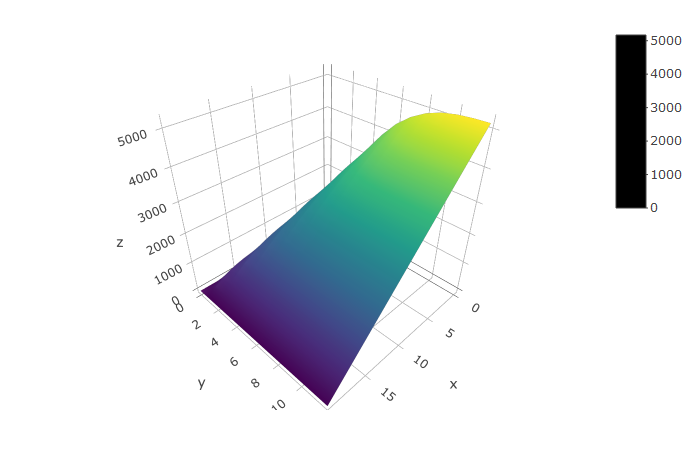
\includegraphics[width=\linewidth]{C:/Users/Stefan/LRZ Sync+Share/Masterarbeit-Klein/Code/Results/smallTest2-False-DP-190619-1333/value_function.png}
\end{figure}

Two issues make ES difficult in practice as pointed out e.g. in \cite{Koch.2017}. First, the decision problem inherent at each state (time period $t$ together with capacity $\boldsymbol{c}$) is an assortment optimization problem over $2^n$ possible offer sets. 
\todo{Ergänze Machbarkeitsanalyse in Tabellenform (Speicherbedarf plus Rechenzeit), s. hierzu VL-Unterlagen Künstl. Intelligenz}
So our small example given by \Cref{tb:AirDesc:Prod} leads to $2^6 = 64$ offer sets.
\todo{Kann das im Cache gespeichert werden (Python und Betriebssystem)}
Second, for each time period $t$, the value function \Cref{eq:Bellman} has to be computed for all possible capacities, which becomes computationally cumbersome due to multi-dimensionality ($m$ resources). In general, $\prod_{h \in [m]} (c^0_h+1)$ instances have to be solved\footnote{The capacity of each resources can take values in $\{0, 1, \dots, c^0_h\}$}. Already our small example given by \Cref{tb:AirDesc:Res} leads to a total of $9\cdot 5\cdot 5\cdot 9 = 2.025$ instances.


\subsection{Choice based linear programming}

Because of the challenges for the exact solution as stated above, approximations are needed to solve \Cref{eq:Bellman}. based on Bront et al and van Ryzin. A popular approach is to approximate the stochastic quantities (purchase probabilities) by deterministic values such as their expected value and to allow capacity and demand to be continuous. This approach is named \emph{Choice based linear programming} (CDLP\nomenclature{CDLP}{choice-based linear program}) and is used by e.g. \cite{GGallego.}, \cite{Liu.2008} or \cite{Bront.2009}.

Taking an eagle-eye perspective, the company has to decide which sets to offer in every single time period. But as purchase probabilities don't change over time, the specific time period when to offer an individual set is indistinguishable, we can aggregate over time. We introduce a few more notation to get a hand on this and keep it close to what is established in the literature. As already stated in \Cref{sss:DCM}, $p_{\boldsymbol{x}}(j)$ can be interpreted as the deterministic quantity of product $j$ being sold in one time period. Let $R(\mathbf{x})$ represent the expected (thus deterministic) revenue given offer set $\boldsymbol{x}$ (again per time period), and let $\boldsymbol{Q}(\boldsymbol{x}) = (Q_1(\boldsymbol{x}), \dots, Q_m(\boldsymbol{x}))^T$ denote the expected capacity being used (also per time period), i.e.

\todo{Layout: Satzzeichen (Punkt oder Komma) ans Ende der Formeln}
\begin{align}
R(\boldsymbol{x}) &= \sum_{j \in [n]} r_j p_{\boldsymbol{x}}(j)\\
Q_h(\boldsymbol{x}) &= \sum_{j \in [n]} a_{hj} p_{\boldsymbol{x}}(j) \quad \forall h \in [m]\quad.
\end{align}

We can denote the total time\footnote{Total time meaning number of time periods.} for which set $\boldsymbol{x}$ is offered by $t(\boldsymbol{x})$ and the set of all possible offersets as $N = \{0,1\}^n$ . Thus, we can formulate the choice-based linear program $V^{CDLP}(T, \boldsymbol{c})$\footnote{Note that in our formulation, $p_{\boldsymbol{x}}(j)$ already includes the parameter for the arrival rate $\lambda$ and thus, $\lambda$ doesn't appear directly in our formulation of the CDLP in contrast to the fomulation in \cite{Bront.2009}.}. Here, the optimization problem is solved by varying the decision variables $t(\boldsymbol{x})$. 

\begin{align}
V^{CDLP}(T, \boldsymbol{c}): \qquad\qquad & \max \sum_{\boldsymbol{x}\in N} R(\boldsymbol{x}) t(\boldsymbol{x})\\
\text{s.t. } & \sum_{\boldsymbol{x}\in N} Q_h(\boldsymbol{x}) t(\boldsymbol{x}) \leq c_h \quad, \forall h \in [m]\label{eq:CDLP-m}\\
& \sum_{\boldsymbol{x}\in N} t(\boldsymbol{x}) \leq T~,\label{eq:CDLP-1}\\
& t(\boldsymbol{x}) \geq 0 \quad \forall \boldsymbol{x} \in N~.
\end{align}

We want to mention some characteristics of this optimization problem. By allowing $t(\boldsymbol{x})$ to be continuous\footnote{E.g., $t(\boldsymbol{x})=1.2$ corresponds to offerset $\boldsymbol{x}$ being offered for one whole time period and $20\%$ of another time period.}, we arrive at a classical linear program (LP\nomenclature{LP}{linear program}), for which efficient solution methods exist (Simplex) and \todo{Sprache: Hier bezieht sich implemented auf die eben eingeführten solution methods} are implemented (e.g. in Gurobi). Even though the number of variables is exponential ($2^n$ as $N = \{0,1\}^n$), methods such as column-generation techniques can be used to solve this LP efficiently as \cite{GGallego.} and \cite{Liu.2008} show\footnote{Note that Gurobi is high-level and thus programmed in such way so that it realizes which method shall be used to solve a given LP efficiently.}\todo{Verify Gurobi being high-level}. Also note that the optimization problem $V^{CDLP}(T, \boldsymbol{c})$ has $m+1$ constraints ($m$ in \Cref{eq:CDLP-m} and $1$ in \Cref{eq:CDLP-1}). By duality theory and especially Complementary Slackness (compare e.g. to \cite{Domschke.2015}), at most $m+1$ basic variables will end up being non-zero. Hence, even though the number of variables being exponentially large ($2^n$), only a linear number will make up \todo{Sprache: make up}the solution ($m+1$), which again motivates to use column-generation techniques.

The dual of the CDLP is given by
\begin{align}
	\min &\boldsymbol{\pi}^T \boldsymbol{c} + \sigma T\\
	\text{s.t.} &\boldsymbol{\pi}^T \boldsymbol{Q}(\boldsymbol{x}) + \sigma \geq R(\boldsymbol{x}) \quad \forall \boldsymbol{x}\in N\\
	& \boldsymbol{\pi} \geq 0\\
	& \sigma \geq 0 ~,
\end{align}
where $\boldsymbol{\pi}$ is the vector of dual prices corresponding to the resource constraints \Cref{eq:CDLP-m} and $\sigma$ is the dual price corresponding to the time constraint \Cref{eq:CDLP-1}. Again with theory of duality in mind, the optimal value of $\pi_h$ estimates the marginal value of resource $h$ and the optimal value of $\sigma$ provides a marginal value of time (i.e. one additional time period would lead to an expected increase in revenue of $\sigma$ units).

In our small example, there are $256 = 2^8$ offersets

Korrektheit getestet mit \texttt{C:\textbackslash{}Users\textbackslash{}Stefan\textbackslash{}LRZ Sync+Share\textbackslash{}Masterarbeit-Klein\textbackslash{}Code\textbackslash{}H\_CDLP\_single\_leg.py} - Example0 in settings
Ergebnisse in \texttt{ C:\textbackslash{}Users\textbackslash{}Stefan\textbackslash{}LRZ Sync+Share\textbackslash{}Masterarbeit-Klein\textbackslash{}Code\textbackslash{}Results\textbackslash{}example0-False-CDLPSingleLeg-190621-1808}


\clearpage
\setcounter{page}{1}
\noindent\fbox{\parbox{\textwidth}{\centering 27.8.}}

\section{Approximate Dynamic Programming}

\subsection{Approximate Policy Iteration}

ADP builds upon \Cref{eq-DP-optOffer} and approximates opportunity costs additively using bid prices $\pi_h(t, c_h)$, i.e. $\Delta_j V^{t+1}(\boldsymbol{c}) = \sum_{h \in [m]} a_{hj}\pi_{h}(t+1, c_h)$. Thus, the policy is given as the solution of

\begin{align}
^\pi \boldsymbol{x}^t = \argmax_{x^t \in \{0,1\}^n}\left\{ \sum_{j \in [n]} p_j(x_t) \left( r_j - \sum_{h \in [m]} a_{hj}\pi_{h}(t+1, c_h) \right) \right\} 
\end{align}

Thus, the policy is completely described by the bid prices $\pi_h(t, c_h) \forall t$.

Let us discuss the algorithm in depth. In the beginning (\Cref{alg-API1}), all parameters are set to zero which results in the greedy policy of offering the set resulting in the highest expected revenue (no consideration of costs). 

In each policy iteration $k$, the current policy is evaluated first. To do so, we use the current policy to evaluate $I$ random paths. \Cref{alg-API3} sets up the dataset for revenues to go $\hat{V}_t^i$ and remaining capacities $\mathbf{\hat{C}}_t^i$ for all times $t$ and sample paths $i$. 

For each sample path $i$, a storage unit for revenue $\hat{r}_t$ and capacities $\mathbf{\hat{c}}$ is created for all times $t$ (\Cref{alg-API5}). Furthermore, the capacity is set to the initial capacity in \Cref{alg-API6}.

For each point in time, the current capacity $\mathbf{\hat{c}}_t$ is stored in \Cref{alg-API8}, the current bid prices are calculated in \Cref{alg-API9} and used to determine the offerset $\mathbf{x}$ in \Cref{alg-API10}. More details on the determination of the offerset can be found in \Cref{sec-determineOfferset}. With, this, a sales event $j'$ is simulated and in case a product has been sold, the revenue is stored and capacity adjusted (note: the revenue thus belongs to $t$ and capacity will affect $t+1$) (\Cref{alg-API11} to \Cref{alg-API13}).

After simulating one sample path, the value function for this sample path $\hat{V}_t$ is updated for all times $t$ in \Cref{alg-API14}, and so are the capacities in line \Cref{alg-API15}.

With all the information from the $I$ sample paths the parameters $\left(\theta_t, \pi_t \right)$ are updated. Note that the old parameters are used as starting values and the current number of policy iterations $k$ is also passed to potentially take care of exponential smoothing. Thus, we have $(1+h)*T$ parameters ($theta_t$ and $\pi_t$) and $2TI$ data points. More details on the update of the parameters can be found in \Cref{sec-updateParameter}.

%TODO Visualisierung wann was stattfindet
Actions possible in $t = 0, \dots, T-1$.


\begin{algorithm}
	\caption{Approximate policy iteration}\label{alg-API}
	\begin{algorithmic}[1]
		\State Set $\theta_t = 0$ and $\mathbf{\pi}_t = \mathbf{0}$ $\forall t = 0, \dots, T-1$ \label{alg-API1}
		\For{\texttt{k = 1 to K}} \label{alg-API-Piter1}
		\State Set $\hat{V}_t^i = 0$ and $\mathbf{\hat{C}}_t^i = 0$ $\forall t = 0, \dots, T-1, \forall i = 1, \dots, I$\label{alg-API-Piter2}\label{alg-API3}
		\For{\texttt{i = 1 to I}}\label{alg-API-Peval1}
		\State Set $\hat{r}_t = 0$ and $\mathbf{\hat{c}}_t = 0$ $\forall t = 0, \dots, T-1$\label{alg-API5}
		\State Initialize $\mathbf{c} = \mathbf{c}^0$\label{alg-API6}
		\For{\texttt{t = 0 to T-1}}
		\State $\mathbf{\hat{c}}_t \coloneqq \mathbf{c}$\label{alg-API8}
		\State Compute $\mathbf{\pi}(t, \mathbf{c})$ \label{alg-API-calcPi}\label{alg-API9}
		\State Compute $\mathbf{x} = \text{determineOfferset}(\mathbf{\pi}(t, \mathbf{c}), \epsilon_t)$\label{alg-API10}
		\State Simulate a sales event $j' \in \{0, 1, \dots, n\}$\label{alg-API11}
		\If{$j' \in \{ 1, \dots, n\}$}
		\State $\hat{r}_t = r_{j'}$ and $\mathbf{c} = \mathbf{c} - \mathbf{a}_{j'}$\label{alg-API13}
		\EndIf
		\EndFor
		\State Compute $\hat{V}_t^i = \sum_{\tau = t}^{T}\hat{r}_t \quad \forall t = 0, \dots, T-1$\label{alg-API14}
		\State Assign $\mathbf{\hat{C}}_t^i = \mathbf{\hat{c}}_t \quad \forall t = 0, \dots, T-1$\label{alg-API15} \label{alg-API-Peval2}
		\EndFor
		\State $\left(\theta_t, \pi_t \right) = \text{updateParameters}\left(\hat{V}_t^i, \mathbf{\hat{C}}_t^i, \theta_t, \pi_t, k\right) \quad \forall t = 0, \dots, T-1, \forall i = 1, \dots, I$ \label{alg-API-updateParam}\label{alg-API-Piter3}
		\EndFor
		\Return {$\left(\theta_t, \pi_t \right)  \quad \forall t = 1, \dots, T$}
	\end{algorithmic}
\end{algorithm}


Overview of parameters:
\begin{enumerate}
	\item $\theta_t$	optimization parameter (offset)
	\item $\mathbf{\pi}_t$	optimization parameter (bid price for each resource)
	\item $\hat{V}_t = 0$	all sample revenues to go for each sample for each time
	\item $\mathbf{\hat{C}}_t = 0$	all sample available capacities for each sample for each resource for each time
	\item $r_t$	sample revenue generated at time $t$
	\item $\mathbf{c}$	available capacities for each resource at current time
	\item $\mathbf{c}^0$	starting capacities
	\item $\mathbf{x}$ offerset at current time
	\item $\epsilon_t$ epsilon used at current time
\end{enumerate}





\clearpage
\section{Old-Already written}

\subsection{Dynamic Programming - Theory}

As this whole thesis is based on the ideas of Dynamic Programming, we want to give a short overview of the underlying mathematical theory and directly combine it to our setting.

Dynamic Programming (DP\nomenclature{DP}{dynamic programming}) refers to a broad collection of algorithms used to compute optimal policies given a perfect model of the environment as a Markov Decision Process (MDP\nomenclature{MDP}{markov decision process}), as stated in \cite{Sutton.2018}. A MDP is characterized by a state set $\mathcal{S}$ (the varying capacities $\mathbf{c}$ together with the current point in time $t$), an action set $\mathcal{A}$ (the offer sets $\mathbf{x}$) and reward sets $\mathcal{R}$ (the revenue $r$ if a product is sold). A MDP evolves over time, but for the evolution from time $t$ to $t+1$ only the current state $s_t$ is relevant and the history of previous states $s_h, h<t$ can be ignored. The dynamic is given by a set of probabilities $p(s', r | s, a)$ (capacities reduce according to which random product the random customer has bought according to his preferences). 

The goal of DP is to determine the optimal policy, i.e. which action to choose at each given state. Key to the solution is the usage of value functions as seen above. These fulfil the Bellman optimality equations as stated in \Cref{eq-Bellman}. 

%TODO elaborate on curse of dimensionality
In our setting, uniqueness of the optimal value function is ensured, as the MDP is guaranteed to terminate under any policy because time is moving forward no matter which action we choose, compare \cite{Sutton.2018}. Thus, while the problem can be solved, due to large scale decision problems and the curse of dimensionality, we are lacking computing power to solve it exactly and have to come up with approximate solution methods.

One approximate solution method is the usage of Approximate Policy Iteration (API\nomenclature{API}{approximate policy iteration}), which consists of two steps. The policy evaluation step (inner loop \Cref{alg-API-Peval1} to \Cref{alg-API-Peval2}) evaluates a fixed policy over a set of sample paths $\omega_i, i = 1, \dots, I$. The policy improvement step (outer loop \Cref{alg-API-Piter1}, \Cref{alg-API-Piter2}, \Cref{alg-API-Piter3}) improves the policy over the iterations $k = 1, \dots, K$.




\section{Approximate Dynamic Programming}

\subsection{Approximate Policy Iteration}


\subsection{Greedy Heuristic to determine offerset}\label{sec-determineOfferset}

The following algorithm is based on the ideas of the greedy heuristic for the column generation subproblem outlined in \cite{Bront.2009}.

Our goal is to determine a reasonable set of products to offer in a fast manner. Thus, we use a heuristic and cut down the amount of products to consider as fast as possible.

%todo expand on exploration vs exploitation dilemma
The function $\text{determineOfferset}(\mathbf{\pi}, \epsilon)$ calculates the set to offer depending on the current bid prices $\mathbf{\pi}$ via the greedy algorithm layed out in \cite{Bront.2009}. To account for the exploration vs exploitation dilemma, an epsilon-greedy strategy is used. With a probability of $\epsilon/2$ either no product is offered at all or all products with positive contribution $r_j - \sum_{h \in [m]} a_{hj} \cdot \pi_h$ are offered. With a probability of $1-\epsilon$, the proper calculated set is offered.

\todoRed{Value Funktion gebuendelt dargestellt und ueberall mit $\lambda$. Vergleiche zu Bront et al. 4.2.2, wo in 3. ohne $\lambda$ und in 4.a mit $\lambda$.}

\begin{algorithm}
	\caption{Greedy Heuristic}\label{alg-GreedyHeuristic}
	\begin{algorithmic}[1] % [1] results in line numbers
		% Großes X verwendet, um Menge zu symbolisieren
		\State $\text{Value}(X) \coloneqq \sum_{l=1}^{L} \lambda_l \frac{\sum_{i \in X}(r_i - A_i^T\pi)u_{li}}{\sum_{i \in X}u_{li} + u_{l0}}$
		\State $S\coloneqq \emptyset,\quad S' \coloneqq \left\{j \in N : r_j - A_j^T\pi > 0\right\}$ \label{alg-L1}
		\State $j^* \coloneqq \arg\max_{j \in S'} \text{Value}(\{j\})$
		\Repeat
		\State $S \coloneqq S \cup \{j^*\},\quad S' \coloneqq S'\backslash\{j^*\}$
		\State $j^* \coloneqq \arg \max_{j \in S'} \text{Value}(S \cup \{j\})$
		\Until {$\text{Value}(S \cup \{j^*\}) \leq \text{Value}(S)$\\}
		\Return {$S$}
	\end{algorithmic}
\end{algorithm}

%todo Kommentiere den Algorithmus.
Let $S'$ be the set of products with positive reduced costs, i. \Cref{alg-L1}

\subsection{Update of parameters}\label{sec-updateParameter}
%todo Schreibweise der Funktion anpassen, da alle Parameter auf eimal übergeben werden, und nicht separat je Zeitschritt
The function $\left(\theta_t, \pi_t \right) = \text{updateParameters}\left(\hat{V}_t, \mathbf{\hat{C}}_t, \theta_t, \pi_t, k\right)$ really optimizes the following least squares optimization problem for all parameters ($t = 1, \dots, T$) at the same time.

\begin{align}
V_t(\theta_t, \mathbf{\pi}_t, \mathbf{c}_t) & \coloneqq \theta_t + \sum_{h=1}^{m}\sum_{s=1}^{S_h} \pi_{ths} f_{hs}(c_h) \\
f_{hs}(c_h) &\coloneqq 
\begin{cases}\label{def-f}
0 & \text{ if } c_h \leq b_h^{s-1}\\
c_h - b_h^{s-1} & \text{ if } b_h^{s-1} < c_h \leq b_h^s \\
b_h^s - b_h^{s-1} & \text{ if } b_h^s < c_h
\end{cases}
\end{align}

\Cref{def-f} describes the occupied amount of capacity of interval $\left(b_h^{s-1}, b_h^s\right]$.

The following optimization problem depends on the old parameters $\theta_t = \theta_t^k$ and $\mathbf{\pi}_t = \mathbf{\pi}_t^k$ to determine the optimal parameter $\theta_t^{update}$ and $\mathbf{\pi}_t^{update}$.

\begin{alignat}{2}
& \text{min} \sum_{i=1}^{I}\sum_{t=1}^{T} \left( \hat{V}_t^i - V_t(\theta_t, \mathbf{\pi}_t, \mathbf{c}_t^i) \right)^2 && \\
& s.t. && \\
& \theta_t \geq 0 && \forall t\\
& \max_{j=1, \dots, n} r_j \geq \pi_{ths} \geq 0 && \forall t, h, s\\
& \pi_{ths} \geq \pi_{th,s+1} && \forall t, h, s = 1, \dots, S_h-1\\
& \theta_t \geq \theta_{t+1} && \forall t = 1, \dots, T-1\\
& \pi_{ths} \geq \pi_{t+1,hs} && \forall t = 1, \dots, T-1
\end{alignat}

The final parameters $\theta_t^{K+1}$ and $\mathbf{\pi}_t^{K+1}$ can obtained via two possible equally possible ways. One is the so called exponential smoothing, where in each iteration $k$ the parameter for the next iteration $k+1$ is calculated via:
\begin{align}
\theta_t^{k+1} &= \left(1- \frac{1}{k} \right)	\theta_t^k + \frac{1}{k} \theta_t^{update}\\
\mathbf{\pi}_t^{k+1} &= \left(1- \frac{1}{k} \right)	\mathbf{\pi}_t^k + \frac{1}{k} \mathbf{\pi}_t^{update}
\end{align}
The other one uses $\theta_t^{k+1} = \theta_t^{update}$ and $\mathbf{\pi}_t^{k+1} = \mathbf{\pi}_t^{update}$ and averages at the very end.
\begin{align}
\theta_t^{K+1} &= \frac{1}{K}\sum_{k=1}^{K}\theta_t^k\\
\mathbf{\pi}_t^{K+1} &= \frac{1}{K}\sum_{k=1}^{K}\mathbf{\pi}_t^k
\end{align}

\begin{proof}
	\todoMinor{Den Beweis sauber ausfuehren. Hier sind die Inhalte. Die Aussage stimmt, falls die gefundenen optimalen Loesungen in jeder Iteration stets dieselben sind. Dies ist der Fall, wenn es stets nur ein Minimum gibt. Wir haben eine quadratische Zielfunktion, die sozusagen eine mehrdimensionale, nach oben geoeffnete Parabel zeigt, die genau ein globales Minimum besitzt. Weitere noetige Punkte: eindeutiges globales Minimum ueber positiv definite Hesse-Matrix. Optimum auch zulaessig (schwierig?)}
\end{proof}




\noindent\rule{\textwidth}{1pt}
\subsection{More stuff}
Calculations:
$\mathbf{\pi}(t, \mathbf{c}) = \pi_h(t, c_h) \text{ for } h \in [m]$

\begin{numcases}{\pi_h(t, c_h) = }
\infty & if $c_h = 0$ \\
\sum_{s=1}^{S_h} \pi_{ths}\mathbbm{1}_{\left(b_h^{s-1}, b_h^s\right]}(c_h) &  otherwise.
\end{numcases}

\todoRed{Fuer \Cref{alg-API-calcPi} verwende Zeit \textbf{t} statt \textbf{t+1}. Grund: Kenne Informationen zur Zukunft nicht.}



\noindent\rule{\textwidth}{1pt}
A sales event is simulated by first having one or zero customer arrive at random. In case a customer arrives, its preference function given the offer set determines the probability according to which one product is sold ($j' \in \{1, \dots, n\}$) or no product is sold ($j' = 0$).



\subsection{Thoughts on implementation}

This shall be a short overview of my thoughts regarding the implementation:

\begin{enumerate}
	\item I wanted to produce reproducible results, i.e. my code shall be usable on a larger scope. Logic and Settings shall be separated. Completed code shall be script based and after run, create a folder with its running configuration.
	\item Be careful, when storing list or dataframes, as a deepcopy might have to be used.
	\item 
\end{enumerate}
\chapter{Comparison}

Our goal is to evaluate different policies. One policy is considered better then another policy if it generally leads to higher total revenues. To put this vague phrasing into a scientifically sound comparison, we use an approximate two sample test, which we'll describe here in more detail. We base this overview and notation mainly on Ch. 14.7 of \cite{Bamberg.2011} with extensions as in Ch. 11.3 of \cite{Fahrmeir.2007}.

We have a total of $M$ sample paths each consisting of $T$ time steps, i.e. $M \times T$ random numbers determining which customer arrives and $M \times T$ random numbers leading to which product is purchased. Those two numbers are called \textit{exogenous information}. When applying policy $A$, for each sample path at each time step, the respective offerset is presented to the current customer and its preferences determine which product is purchased. All purchases of one sample path are aggregated and stored, such that policy $A$ results in the vector of values $\mathbf{v}^A \in \mathbb{R}^M$. Accordingly, $\mathbf{v}^B$ is determined. As both policies rely on the same exogenous information, the samples are dependent and a paired samples t-test has to be used.

Thus, we end up with two observations of size $M$ 

$$v^A_1, \dots, v^A_M \text{ respectively } v^B_1, \dots, v^B_M~.$$

%todo notation: A once on top and once on bottom
Let $\bar{\mathbf{v}^A}$ and $S_A^2$ resp. $\bar{\mathbf{v}^B}$ and $S_B^2$ be the empirical mean and empirical variance. Furthermore, $\mu^A$ and $\sigma_A^2$ denote the expected value and variance of $v^A_i$, respectively $\mu^B$ and $\sigma_B^2$ denote the expected value and variance of $v^B_i$. The hypothesis that policy $A$ is better then policy $B$ results in the following null and alternative hypothesis:

$$H_0: \mu^A \leq \mu^B, H_1: \mu^A > \mu^B$$




\bibliography{bibliography}
\end{document}
